\documentclass[12pt, sumario=abnt-6027-2012, openright, oneside, a4paper, english, brazil, chapter=TITLE, section=TITLE]{abntex2}
\RequirePackage{uva}

% Informações do Curso
\instituicao{Universidade Estadual Vale do Acaraú - UVA}
\centro{Centro de Ciências Exatas e Tecnologia - CCET}
\curso{Curso de Ciências da Computação}
\coordenador[Coordenador do Curso]{Nome do Coordenador}

% Informações do Trabalho
\autor{Nome do autor}
\titulo{Título do trabalho}
\subtitulo{Subtítulo, se houver} % Se não houver subtítulo, deixar vazio
\tipotrabalho{Monografia}
\grau{Bacharel em Ciências da Computação} % Ex.: Bacharel em Ciências da Computação

% Orientadores (No caso de Orientadora, ou Coorientadora, alterar os nomes entre colchetes
\orientador[Orientador:]{Nome do orientador}
\coorientador[Coorientador:]{Nome do coorientador} % Se não houver, deixar o conteúdo entre chaves vazio

% Banca Avaliadora - Caso a banca seja formada apenas por três avaliadores, incluindo o orientador, deixar as
% informações referentes à bancac vazias. \bancac{}{}
\bancao{\imprimirorientador}{UVA}
\bancaa{Nome do 1o. avaliador, Titulo}{Instituição 01}
\bancab{Nome do 2o. avaliador, Titulo}{Instituição 02}
\bancac{Nome do 3o. avaliador, Titulo}{Instituição 03} 

% Local e Ano
\local{Sobral}
\data{Ano}

% Palavras-chave - Preencher as que forem necessárias {Português}{Língua estrangeira}. Deixar as outras vazias
\pca{Palavra1}{Word1}
\pcb{Palavra2}{Word2}
\pcc{Palavra3}{Word3}
\pcd{Palavra4}{Word4}
\pce{Palavra5}{Word5}
\pcf{}{}

\pgfplotsset{compat=1.16}

\makeindex

\begin{document}
    \pretextual
        \imprimircapa
        \imprimirfolhaderosto
        \imprimirfolhaaprov
        \imprimirdedicatoria{Escreva aqui a sua dedicatória ... }
        \imprimiragradecimentos % arquivo capitulos/agradecimentos.tex
        \imprimirepigrafe{Escreva aqui uma frase, de preferência relacionada ao seu trabalho, indicando o autor.}{Autor}
        \imprimirresumolv % Resumo em lingua vernácula: arquivo capitulos/resumolv.tex
        \imprimirresumole{english}{Abstract}{Keywords} % Resumo em língua estrangeira - arquivo capitulos/resumole.tex

        \listadefiguras     % ambiente figure*
        \listadegraficos    % ambiente graphic
        \listadequadros     % ambiente board
        \listadetabelas     % ambiente table*
        %\listadealgoritmos  % ambiente algorithm
        \listadesiglas       % arquivo capitulos/siglas.tex
        \listadesimbolos     % arquivo capitulos/simbolos.tex
        \imprimirsumario

    \textual
        % criar um arquivo para cada um dos outros capítulos, e inserir nos moldes a seguir
        \chapter{Introdução}\label{chp:intro}

\section{Contextualização}

O crescimento da utilização da Internet nos últimos anos tem levado os Provedores de Serviços de Internet (ISPs, \textit{Internet Service Providers}) a buscar soluções capazes de garantir a qualidade dos serviços oferecidos aos usuários. O acesso à rede de um ISP, geralmente, constitui uma etapa preliminar para o acesso ao núcleo da Internet \cite{kalmanek2010guide}. Nesse contexto, diferentes usuários e aplicações apresentam requisitos distintos de comunicação, como largura de banda, latência, disponibilidade e confiabilidade.  Dessa forma, os ISPs precisam disponibilizar recursos capazes de atender aos diferentes requisitos estabelecidos para a prestação de seus serviços.

Esses requisitos podem ser estabelecidos por meio de um acordo de nível de serviço (SLA, \textit{Service Level Agreement}), que define as condições acordadas entre o cliente e o ISP para a prestação de determinado serviço. O cumprimento dessas condições está diretamente relacionado à Qualidade de Serviço (QoS, \textit{Quality of Service}) oferecida pelo provedor e pode influenciar a Qualidade de Experiência (QoE, \textit{Quality of Experience}) percebida pelo usuário. Quando os requisitos estabelecidos não são atendidos, a qualidade do serviço pode ser comprometida, resultando em problemas como lentidão e atrasos na comunicação \cite{gomes2020strategies,foukas2017network}.

A necessidade de recursos por parte dos usuários não permanece constante ao longo do tempo. Diferentes períodos podem apresentar variações na quantidade de solicitações e na utilização da infraestrutura, fazendo com que a demanda por recursos da rede aumente ou diminua de acordo com as necessidades dos usuários e das aplicações. Em uma infraestrutura compartilhada, essa característica torna o gerenciamento dos recursos mais complexo, pois uma capacidade dimensionada para atender aos períodos de maior demanda pode permanecer subutilizada em momentos de menor utilização, enquanto uma capacidade insuficiente pode comprometer o atendimento dos usuários durante períodos de maior demanda. Dessa forma, torna-se necessário utilizar os recursos disponíveis de maneira eficiente, adaptando sua distribuição às diferentes condições de demanda.

Nesse contexto, o fatiamento de redes surge como uma abordagem capaz de utilizar uma mesma infraestrutura física para criar diferentes redes virtuais, denominadas fatias, que podem ser configuradas de acordo com os requisitos específicos de cada serviço ou aplicação \cite{vassilaras2017algorithmic}. Dessa forma, os recursos físicos da infraestrutura podem ser compartilhados entre diferentes fatias, permitindo que cada uma possua características e recursos adequados às necessidades dos usuários. Essa flexibilidade possibilita uma utilização mais eficiente da infraestrutura, especialmente em cenários nos quais a demanda por recursos apresenta variações ao longo do tempo.

\section{Problema}

A utilização do fatiamento de redes permite que os recursos de uma infraestrutura física sejam compartilhados entre diferentes fatias, de acordo com os requisitos de cada serviço ou aplicação. Entretanto, a definição de como esses recursos devem ser distribuídos entre as fatias constitui um desafio, especialmente em ambientes nos quais a demanda varia ao longo do tempo. Nesse cenário, diferentes estratégias podem ser utilizadas para determinar quais recursos serão alocados, quais fatias serão reutilizadas e quando uma nova busca por recursos deve ser realizada.

Diferentes estratégias podem ser adotadas para realizar essa alocação e adaptar as fatias às variações nas necessidades dos usuários ao longo do tempo. \citeonline{gomes2020strategies} comparam estratégias de fatiamento elástico e mostram que a política utilizada afeta métricas como disponibilidade de banda e quantidade de clientes atendidos. Este estudo delimita-se à comparação, sob as mesmas requisições e topologias, do PETIC, de duas buscas aproximadas para seu custo aditivo (ACO e Q-Learning) e do SA, cuja função objetivo inclui equilíbrio de carga.

A questão de pesquisa é: \textbf{como variam a aceitação de demandas, o equilíbrio da utilização dos enlaces, a reutilização de caminhos e o tempo de decisão dessas quatro implementações em diferentes níveis de carga e topologias, quando avaliadas nos mesmos cenários independentes?} São examinadas as seguintes hipóteses: (H1) as diferenças de aceitação entre PETIC, ACO e Q-Learning podem variar por cenário e não se presume uma ordenação entre eles; (H2) a função multiobjetivo do SA favorece maior equilíbrio dos enlaces, potencialmente acompanhado de caminhos mais longos e menor aceitação sob carga alta; (H3) a busca exata por Dijkstra no PETIC requer menos tempo de CPU que as buscas estocásticas avaliadas. As hipóteses são avaliadas por métricas comuns e, para aceitação, por diferenças pareadas por cenário. Como ACO e Q-Learning aproximam o mesmo custo aditivo já minimizado pelo PETIC, este trabalho não testa se superam o ótimo desse custo; investiga como os mecanismos de busca se refletem nos resultados da alocação sequencial.

\section{Justificativa}

A análise comparativa de diferentes estratégias de fatiamento permite compreender como suas características influenciam a utilização dos recursos disponíveis em diferentes condições da rede. \citeonline{gomes2020strategies} demonstram que estratégias distintas podem favorecer diferentes aspectos da infraestrutura, como disponibilidade de banda, saturação dos recursos e quantidade de clientes atendidos. Essa análise torna-se especialmente relevante em ambientes de demanda elástica, nos quais as necessidades de recursos podem variar ao longo do tempo. Nesse cenário, conhecer as vantagens e limitações de cada estratégia pode contribuir para a escolha de abordagens mais adequadas às diferentes condições de utilização da infraestrutura.

Em um ambiente de demanda elástica, a avaliação dessas estratégias sob diferentes condições de utilização torna-se importante, pois o comportamento da rede pode se modificar à medida que a demanda aumenta ou diminui. Uma estratégia que apresenta resultados satisfatórios em determinado nível de utilização pode não manter o mesmo comportamento diante de outras condições de demanda. Dessa forma, a realização de experimentos que considerem essas variações possibilita uma análise mais ampla do desempenho dos algoritmos, evitando que sua avaliação seja limitada a um único cenário.

A comparação entre diferentes algoritmos de fatiamento pode contribuir para uma melhor compreensão das características de cada abordagem e dos cenários nos quais sua utilização se mostra mais adequada. A identificação desses comportamentos permite observar não apenas qual estratégia apresenta melhores resultados em determinada condição, mas também quais fatores podem influenciar seu desempenho. Dessa forma, estudos comparativos podem contribuir para o desenvolvimento e aprimoramento de mecanismos de alocação de recursos em ambientes de demanda elástica.
% RASCUNHO PRELIMINAR redigido com apoio de IA (Claude Code, Anthropic; ver ficha de uso de IA).
% A interpretação é uma proposta de leitura dos dados e deve ser revisada, validada e reescrita pelo autor.
\section{Objetivos}

Considerando o problema apresentado, este trabalho busca analisar diferentes algoritmos de fatiamento de redes em cenários de demanda elástica, de forma a compreender suas características e diferenças de desempenho.

\subsection{Objetivo Geral}

Este trabalho tem como objetivo geral implementar um simulador reprodutível de alocação de fatias e comparar o PETIC, o ACO, o Q-Learning e o SA em diferentes topologias e níveis de demanda, caracterizando as diferenças observadas sem presumir superioridade por aceitação.

\subsection{Objetivos Específicos}

\begin{itemize}
    \item analisar o comportamento dos algoritmos de fatiamento selecionados diante de diferentes condições de demanda;
    
    \item comparar o desempenho dos algoritmos a partir dos resultados obtidos nos experimentos;
    
    \item identificar as características, vantagens e limitações apresentadas por cada abordagem nos cenários avaliados;
    
    \item disponibilizar a configuração, os dados de execução e os scripts de análise para reprodução dos resultados.
\end{itemize}

\subsection{Contribuições Científicas e Delimitação}

A contribuição científica deste trabalho não consiste na proposição de um novo algoritmo ou protocolo de alocação de fatias de rede, mas na condução de uma avaliação comparativa empírica e reprodutível de quatro implementações completas (o algoritmo determinístico PETIC, as meta-heurísticas ACO e SA, e o algoritmo de aprendizado por reforço Q-Learning) sob demandas pareadas e com controle experimental sistemático.

Essa investigação diferencia-se dos trabalhos relacionados na literatura (discutidos na Seção~2.7), que tratam do escalonamento autonômico de réplicas de servidores \cite{pasin2013infaestrutura}, de arquiteturas de gerenciamento e orquestração de fatias \cite{maciel2020gerenciamento}, da alocação de blocos de recursos em redes de acesso 5G Open RAN \cite{limafilho2026controle} ou avaliam políticas de fatiamento elástico sob um único cenário sintético sem delineamento em blocos casualizados \cite{gomes2020strategies}. Em contrapartida, este estudo concentra-se especificamente na seleção e adaptação de caminhos em topologias de transporte em malha com 30 cenários sintéticos independentes por célula e testes estatísticos pareados.

A infraestrutura completa de experimentação — abrangendo o código-fonte do simulador, as sementes, as configurações, os dados brutos e os scripts de análise e visualização — é disponibilizada publicamente em repositório aberto\footnote{Disponível em: \url{https://github.com/chagasduarte/elastic-network-slicing}.}% VERIFICAR: o autor deve confirmar a data de acesso.
. As conclusões apresentadas delimitam-se estritamente às quatro implementações analisadas e às condições experimentais avaliadas, sem pretensão de extrapolação além dos algoritmos e cenários investigados.

% RASCUNHO PRELIMINAR redigido com apoio de IA (Claude Code, Anthropic; ver ficha de uso de IA).
% A interpretação é uma proposta de leitura dos dados e deve ser revisada, validada e reescrita pelo autor.
\section{Organização do Trabalho}

Este trabalho está organizado em cinco capítulos. O Capítulo~\ref{chp:fund_teo} apresenta a fundamentação teórica: a virtualização de redes, as redes definidas por software, a virtualização de funções de rede, o fatiamento de redes, a demanda elástica e os algoritmos de alocação de fatias considerados (PETIC, ACO, SA e Q-Learning). O Capítulo~\ref{chp:metodologia} descreve a metodologia: a caracterização da pesquisa, o ambiente de simulação, o modelo do problema, a implementação e a calibração dos algoritmos, as topologias, os cenários de demanda, as métricas e o procedimento experimental. O Capítulo~\ref{chp:resultados} apresenta e discute os resultados dos experimentos. Por fim, o Capítulo~\ref{chp:conclusao} apresenta as conclusões, as limitações e os trabalhos futuros.


        \chapter{Citações}\label{chp:citacoes}

    Citação é a utilização, no texto que estamos produzindo, de partes de outros trabalhos ou de ideias de outros autores, de preferência reconhecidos como autoridades no assunto tratado. Faz-se a citação para esclarecer algum aspecto particular do tema ou para reforçar um argumento nosso como o ponto de vista do outro autor.

    Existem três tipos de citação:

    \begin{alineas}
        \item \textbf{Direta:} transposição literal de um texto de outro autor, no todo ou em parte.
        \item \textbf{Indireta:} apresentação do conteúdo de um trecho de outro autor, sem transcrição literal.
        \item \textbf{Citação de citação:} citação direta ou indireta de outro autor ao qual não se teve acesso ao original, mas sim através de outra citação.
    \end{alineas}

    A citação direta pode ser curta ou longa. Ela é considerada cursa se no texto original tiver até 3 linhas. Caso contrário, ela é considerada longa. A citação direta curta deve ser feita no próprio texto, entre aspas. Já a longa deve ser feita sem aspas (a menos que estas já façam parte do texto original). com recuo de $4cm$ a partir da margem esquerda, letra menor que a utilizada no texto e espaçamento simples. Para isso, basta utilizar o ambiente \verb| citacao |.

    O exemplo a seguir é uma citação direta curta, cuja informação está na página $2$ do Livro ``Graph Theory'' de Bundy e Murty.

    Segundo \citeonline[p. 2]{BondyMurty}, ``\emph{grafos} são assim chamados por poderem ser representados graficamente, e é essa representação gráfica que nos ajuda a compreender muitas de suas propriedades''.

    Em vez do comando \verb| \citeonline |, poderíamos ter utilizado o comando \verb| \cite |. O resultado ficaria assim:

    Segundo \cite[p. 2]{BondyMurty}, ``\emph{grafos} são assim chamados por poderem ser representados graficamente, e é essa representação gráfica que nos ajuda a compreender muitas de suas propriedades.''

    A seguir temos um exemplo de citação direta longa, utilizando como referência os mesmos autores anteriores.
  
    \begin{citacao}
        Um \emph{grafo} $G$ é um par ordenado $(V(G),E(G))$ consistindo de um conjunto $V(G)$ de vértices e um conjunto $E(G)$ de arestas, disjunto de $V(G)$, juntamente com uma função de incidência $\psi_G$ que associa um par (não ordenado) de vértices a cada aresta de $G$. Se $e$ é uma aresta, e $u$ e $v$ são os vértices tais que $\psi_G(e) = \{u,v\}$, $u$ e $v$ são as extremidades de $e$. \cite[p.2]{BondyMurty}
    \end{citacao}

    Caso se deseje suprimir partes de uma citação, isso deve ser feito utilizando sinal de reticências entre colchetes. Por Exemplo:

    Por fim, a citação de citação é quando se faz uma citação que já foi feita por outro autor. Por exemplo: Segundo \apudonline[p. 10]{HavetASD}{BondyMurty}, ``Não há uma única maneira correta de se desenhar um grafo''.

    A citação acima poderia ter sido feita também utilizando o comando \verb| \apud |. O que se deseja dizer é que a citação foi feita por Havet e isso consta na página 10 do livro de Bondy e Murty. Esta citação especificamente não foi feita na obra indicada. O exemplo está aqui apenas para ilustração.
        \chapter{Figuras}\label{chp:fig}

    A \cref{fig:figura1} traz uma imagem única, adicionada utilizando o ambiente \emph{figure}.

    \begin{figure}[!htb]
        \centering
        \caption{Figura de exemplo A}
        \label{fig:figura1}
        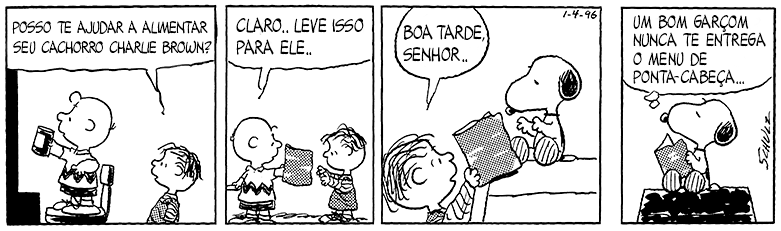
\includegraphics[scale=.5]{figuras/figura1}
        \fonte{Autoria própria.}
    \end{figure}

    Já na \cref{fig:figura2}, temos a mesma figura anterior, mas agora de forma quebrada em subfiguras, usando os ambientes \emph{figure} e \emph{subfigure}. Em \subref{fig:figura2a} temos a primeira parte, em \subref{fig:figura2b} temos a segunda parte, em \subref{fig:figura2c} temos a terceira parte, e em \subref{fig:figura2d} temos a quarta parte da figura. Caso deseje escrever algum rótulo ao lado das letras indicativa de uma subfigura, basta especificá-lo no comando \emph{caption} desta. Para omitir as letras (a), (b), (c) e (d), basta utilizar o comando \emph{caption*} em cada subfigura.

    \begin{figure}[!htb]
        \centering
        \caption{Exemplo de subfiguras}
        \label{fig:figura2}
    
        \begin{subfigure}{.29\textwidth} % Entre chaves, especificar a largura do espaço destinado à subfigura
            \centering
            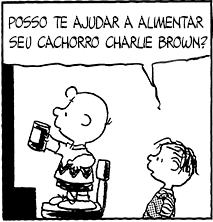
\includegraphics[scale=.5]{figuras/figura2a}
            \caption{}
            \label{fig:figura2a}
        \end{subfigure}
        %
        \begin{subfigure}{.19\textwidth}
            \centering
            
\includegraphics[scale=.5]{figuras/figura2b}
            \caption{}
            \label{fig:figura2b}
        \end{subfigure}
        %
        \begin{subfigure}{.29\textwidth}
            \centering
            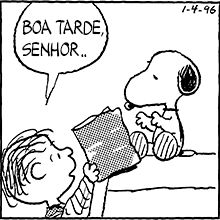
\includegraphics[scale=.5]{figuras/figura2c}
            \caption{}
            \label{fig:figura2c}
        \end{subfigure}
        %
        \begin{subfigure}{.19\textwidth}
            \centering
            
\includegraphics[scale=.5]{figuras/figura2d}
            \caption{}
            \label{fig:figura2d}
        \end{subfigure}
    
        \fonte{Autoria própria.}
    \end{figure}

    A fonte das figuras (e isso também vale para demais elementos como gráficos, tabelas, quadros etc.) deve estar especificada corretamente. Neste modelo, como trata-se apenas de exemplos, todas as fontes estão como ``Autoria própria''.
        \chapter{Gráficos}\label{chp:graficos}

    O \cref{grf:distidadeingr} a seguir traz a distribuição dos alunos ingressantes no Curso de Ciências da Computação por faixa etária.

    \begin{graphic}[htb]
        \caption{Barras}
        \label{grf:distidadeingr}
        \centering
        \begin{tikzpicture}
            \tiny
            \begin{axis}[
                %title = {Distribuição dos Alunos por Faixa Etária},
                %xlabel = {Períodos letivos},
                ylabel = {Qtd. de alunos},
                font =\footnotesize,
                width = 10cm,
                height = 4.9cm,
                ybar =2*\pgflinewidth,
                bar width=8pt,
                ymajorgrids = true,
                symbolic x coords={$2013.1$,$2013.2$,$2014.1$,$2014.2$},
                xtick = data,
                ymin=0,
                ymax=50,
                enlarge x limits=0.25,
                legend cell align=left,
                legend image code/.code={\draw[#1] (0cm,-0.1cm) rectangle (0.2cm,0.1cm); },
                legend style={legend pos=outer north east, column sep=1ex}
                %legend style={at={(1.0,1.15)}, anchor=north,legend columns=-1}
            ]
    
                \addplot[style={cl00,fill=cl01}] coordinates {($2013.1$, 27) ($2013.2$, 30) ($2014.1$, 35) ($2014.2$, 44)};
                \addplot[style={cl00,fill=cl02}] coordinates {($2013.1$, 11) ($2013.2$,  8) ($2014.1$,  5) ($2014.2$,  6)};
                \addplot[style={cl00,fill=cl03}] coordinates {($2013.1$,  0) ($2013.2$,  0) ($2014.1$,  0) ($2014.2$,  1)};
                \addplot[style={cl00,fill=cl04}] coordinates {($2013.1$,  0) ($2013.2$,  1) ($2014.1$,  0) ($2014.2$,  0)};
    
                \legend{$16$ a $20$ anos, $21$ a $25$ anos, $26$ a $30$ anos, Acima de $30$ anos}
            \end{axis}
        \end{tikzpicture}
        \fonte{Autoria própria}
    \end{graphic}

    O \cref{grf:distidadematr} a seguir traz a distribuição dos alunos do Curso de Ciências da Computação, matriculados nos dois últimos anos, por faixa etária.

    \begin{graphic}[htb]
        \caption{Pizza}
        \label{grf:distidadematr}
        \centering
        \begin{tikzpicture}
            \tiny
            \pie[text=legend, color = {cl01,cl02,cl03,cl04}, radius=2]
                {38.62/16 a 20, 39.77/21 a 25, 14.99/26 a 30, 6.62/mais de 30}
        \end{tikzpicture}
        \fonte{Autoria própria}
    \end{graphic}

    O \cref{grf:funcoes} a seguir traz exemplos de plotagem de funções.

    \begin{graphic}[!htb]
        \caption{Funções}
        \label{grf:funcoes}
        \centering
        \begin{tikzpicture}
            \tiny
            \begin{axis}[
                axis y line = center,
                axis x line = middle,
                width = 10cm,
    %           height = 6cm,
                xlabel = $x$,
                ylabel = {$f(x)$},
                legend style={legend pos=outer north east, column sep=1ex}
            ]
    
                \addplot [domain =-20:20, samples=100, color=red ]{x^2 - 9};
                \addlegendentry {$f(x) = x^2 - 9$}
    
                \addplot [domain =-20:20, samples=100, color=blue]{x + 2};
                \addlegendentry {$g(x) = x + 2$}
            \end{axis}
        \end{tikzpicture}
        \fonte{Autoria própria}
    \end{graphic}

    \FloatBarrier

    O \cref{grf:fxetariaanual} traz uma representação em linhas da distribuição dos alunos matriculados, por ano e faixa etária, no Curso de Ciências da Computação.

    \begin{graphic}[!htb]
        \caption{Linhas}
        \label{grf:fxetariaanual}
        \centering
        \tiny
        \begin{tikzpicture}
            \begin{axis}[
                title = {Distribuição dos Alunos por Faixa Etária Anual},
                xlabel = {Anos},
                ylabel = {Qtd. de Alunos},
                font = \footnotesize,
                width = 0.6\textwidth,
                height = 6cm,
                ymajorgrids = true,
                grid style={dotted},
                x tick label style={/pgf/number format/1000 sep=},
                xtick = data,
                ytick = {0,40,80,...,200},
                ymin = 0,
                ymax = 200,
                enlarge x limits = 0.25,
                legend cell align = left,
                legend style={legend pos=outer north east, column sep=1ex}
            ]
                \addplot[mark=square*,line width=2pt,style={cl01}] coordinates {(2011,56) (2012,77) (2013,102) (2014,134)};
                \addlegendentry{16 a 20}
    
                \addplot[mark=o,line width=2pt,style={cl02}] coordinates {(2011,170) (2012,151) (2013,142) (2014,138)};
                \addlegendentry{21 a 25}
    
                \addplot[mark=triangle*,line width=2pt,style={cl03}] coordinates {(2011,73) (2012,66) (2013,55) (2014,52)};
                \addlegendentry{26 a 30}
    
                \addplot[mark=halfsquare*,line width=2pt,style={cl04}] coordinates {(2011,37) (2012,30) (2013,28) (2014,23)};
                \addlegendentry{Acima de 30}
            \end{axis}
        \end{tikzpicture}
        \fonte{Autoria própria}
    \end{graphic}
        \chapter{Tabelas e Quadros}\label{chp:tabquad}

    As tabelas e os quadros facilitam a compreensão do fenômeno em estudo, uma vez que apresentam os dados de modo resumido, oferecendo uma visão geral do assunto.

    A principal diferença entre tabelas e quadros está relacionada ao conteúdo e à formatação. Segundo as Normas de Apresentação Tabular, a informação central de uma tabela é o dado numérico. Todos os outros elementos têm a função de complementá-la e explicá-la. Por sua vez, a Associação Brasileira de Normas Técnicas (ABNT), não específica o tipo de conteúdo a ser incluído em um quadro.

    Com relação a formatação, a tabela apresenta os seguintes elementos: título, cabeçalho, conteúdo, fonte e, se necessário, nota explicativa (geral e/ou específica). É dividida por o mínimo possível de linhas na horizontal e as bordas  laterais não podem ser fechadas. Já o quadro, embora siga especificações semelhantes  (título, fonte, legenda, nota(s) e outras informações necessárias), terá suas laterais fechadas.

    A seguir, temos um exemplo de tabela (\cref{tab:modelo}) e de quadro (\cref{brd:modelo}). A tabela poderia ter as linhas verticais e horizontais intermediárias. A diferença, para efeito de identificação no \LaTeX, é basicamente o tipo de ambiente (\emph{table} para tabela, e \emph{board} para quadro). A estrutura de ambos os elementos é definida com o ambiente \emph{tabular}.

    \begin{table}[!htb]
        \small
        \centering
        \caption{Modelo de Tabela}
        \label{tab:modelo}
        \begin{tabular}{lcccc}                                       \hline
            ÁREAS                 & UNESP & UNICAMP & USP & Total \\ \hline
            Interdisciplinar      &  2    &  2      & 2   &  6    \\ 
            Biológicas e da Saúde &  2    &  2      & 2   &  6    \\ 
            Exatas e Tecnológicas &  2    &  2      & 2   &  6    \\ 
            Humanas e Artes       &  2    &  2      & 2   &  6    \\ \hline
            TOTAL                 &  8    &  8      & 8   & 24    \\ \hline
        \end{tabular}
        \vspace{0.2cm}
        \fonte{Elaborada pelo autor}
    \end{table}

    \begin{board}[!htb]
        \centering
        \caption{Modelo de Quadro}
        \label{brd:modelo}
        \begin{tabular}{|l|c|c|c|c|}                                 \hline
            ÁREAS                 & UNESP & UNICAMP & USP & Total \\ \hline \hline
            Interdisciplinar      &  2    &  2      & 2   &  6    \\ \hline
            Biológicas e da Saúde &  2    &  2      & 2   &  6    \\ \hline
            Exatas e Tecnológicas &  2    &  2      & 2   &  6    \\ \hline
            Humanas e Artes       &  2    &  2      & 2   &  6    \\ \hline
            TOTAL                 &  8    &  8      & 8   & 24    \\ \hline
        \end{tabular}
        \vspace{0.2cm}
        \fonte{Elaborado pelo autor}
    \end{board}

    O \cref{brd:multicol} a seguir traz um exemplo de utilização de mesclagem de colunas (comando \emph{multicol}) e linhas (comando \emph{multirow}). Para utilizar os recursos \emph{multirow} e \emph{multicol}, é necessário incluir os pacotes com estes nomes no preâmbulo do arquivo principal (monografia.tex) ou no arquivo do template (uva.sty)

    \begin{board}[!htb]
        \small
        \centering
        \caption{Modelo de quadro com mesclagem de colunas e linhas}
        \label{brd:multicol}
        \begin{tabular}{|l|c|c|c|c|}                                                              \hline
            \multirow{2}{*}{ÁREAS} & \multicolumn{3}{c|}{INSTITUIÇÃO} & \multirow{2}{*}{TOTAL} \\ \hhline{|~|-|-|-|~|}
            ~                      & UNESP     & UNICAMP  & USP      & ~                       \\ \hline
            Interdisciplinar       &  2        &  2       & 2        &  6                      \\
            Biológicas e da Saúde  &  2        &  2       & 2        &  6                      \\
            Exatas e Tecnológicas  &  2        &  2       & 2        &  6                      \\
            Humanas e Artes        &  2        &  2       & 2        &  6                      \\ \hline
            TOTAL                  &  8        &  8       & 8        & 24                      \\ \hline
        \end{tabular}
        \vspace{0.2cm}
        \fonte{Elaborado pelo autor}
    \end{board}

    O \cref{brd:result} traz um exemplo com texto escrito na vertical. Para isso, é necessário incluir o pacote \emph{rotating}. O efeito pode também ser aplicado a tabelas.

    \begin{board}[!htb]
        \small
        \centering
        \caption{Estudos de Feedback Set em Grafos e Digrafos}
        \label{brd:result}      
        \begin{tabular}{|c|c|l|} \hline
            \textbf{Tipo}                   & \textbf{Algoritmo}            & \textbf{Classe}                       \\ \hline
            \multirow{7}{*}{\begin{sideways}
                                Grafos
                            \end{sideways}} & \multirow{4}{*}{Polinomial}   & Grafos cordais (FVS)                  \\ 
                                            & ~                             & Grafos de intervalo (FVS)             \\ 
                                            & ~                             & Grafos de grau no max 3 (FVS)         \\
                                            & ~                             & Grafos em geral (FES)                 \\ \cline{2-3}
                                            & \multirow{2}{*}{Aproximativo} & Grafos em geral (FVS)                 \\ 
                                            & ~                             & (fator de aprox. 2)                   \\ \cline{2-3}  
                                            & \multirow{1}{*}{Exato}        & Caso geral (FVS) - $O(1.734601^n)$    \\ \hline 
            \multirow{4}{*}{\begin{sideways}
                                Digrafos
                            \end{sideways}}
                                            & Polinomial                    & Digrafos planares (FAS)               \\ \cline{2-3}
                                            & \multirow{2}{*}{Aproximativo} & Torneios bipartidos (FVS e FAS)       \\
                                            & ~                             & (fator de aprox. 2)                   \\ \cline{2-3} 
                                            & \multirow{1}{*}{Exato}        & Caso geral (DFVS) - $O^*(1.9977^n)$   \\ \hline
        \end{tabular}
        \vspace{0.2cm}
        \fonte{Elaborado pelo autor}
    \end{board}

    O \cref{brd:cronograma} a seguir, traz um exemplo de cronograma a ser elaborado para o projeto. Nesse caso, deve-se construir um capítulo apenas para apresentar o cronograma de execução do projeto.

    \begin{board}[!htb]
        \small
        \centering
        \caption{Cronograma}
        \label{brd:cronograma}
        \newcommand{\x}{\cellcolor{gray!40}~}
        \begin{tabular}{|l|c|c|c|c|c|}                                         \hline 
          ETAPA                               & JUL & AGO & SET & OUT & NOV \\ \hline \hline
          Elaboração do projeto               & \x  & \x  & ~   & ~   & ~   \\ \hline
          Revisão bibliográfica inicial       & \x  & \x  & ~   & ~   & ~   \\ \hline
          Estudo do problema e suas variações & ~   & \x  & \x  & ~   & ~   \\ \hline
          Estudo dos algoritmos               & ~   & ~   & \x  & \x  & ~   \\ \hline
          Finalização                         & ~   & ~   & ~   & \x  & ~   \\ \hline
          Apresentação                        & ~   & ~   & ~   & ~   & \x  \\ \hline
        \end{tabular}
        \vspace{0.2cm}
        \fonte{Elaborado pelo autor}
    \end{board}

    \newpage
    O \cref{brd:qtdalunos} a seguir traz a quantidade de alunos por curso da Universidade.

    \begin{board}[!htb]
        \small
        \centering
        \caption{Quantidade de alunos por curso}
        \label{brd:qtdalunos}
        \begin{tabular}{|l|l|r|r|} \hline
            \multirow{2}{*}{CENTRO} & \multirow{2}{*}{CURSO}                & \multicolumn{2}{c|}{ALUNOS} \\ \cline{3-4}
                                    &                                       & QTD.        & \%            \\ \hline
            \multirow{6}{*}{CCET}   & Ciências da Computação                & 300         &  10.00        \\ \cline{2-4}
                                    & Engenharia Civil                      & 250         &   8.33        \\ \cline{2-4}
                                    & Física                                & 400         &  13.33        \\ \cline{2-4}
                                    & Matemática                            & 500         &  16.67        \\ \cline{2-4}
                                    & Química                               & 500         &  16.67        \\ \cline{2-4}
                                    & Tecnologia em Construção de Edifícios & 300         &  10.00        \\ \hline
            \multirow{2}{*}{CCS}    & Educação Física                       & 350         &  11.67        \\ \cline{2-4}
                                    & Enfermagem                            & 400         &  13.33        \\ \hline
            \multicolumn{2}{|r|}{TOTAL}                                     & 3000        & 100.00        \\ \hline
        \end{tabular}
        \vspace{0.2cm}
        \fonte{Autoria própria}
    \end{board}

    \postextual
        \makeatother
        \bibliography{referencias}

        %\apendices % Referenciar com \refapd
            %\chapter{Nome do apêndice}\label{apd:nome}
            %
\includepdf{apendices/apendice.pdf}

        %\anexos % Referenciar com \refanx
            %\chapter{Nome do anexo}\label{anx:nome}
            %
\includepdf{anexos/anexo.pdf}

        % Use os comandos \idxitem{item} e \idxsubitem{subitem}{item} no texto, para criar um índice remissivo
        \printindex
\end{document}